\section{Examples of Tangible User Interfaces}
There is a wide variety of Tangible User Interfaces. Possible applications for TUIs are literally endless. Many systems of TUIs have been explored and published in the past, but still a lot of new ideas are coming up and new applications for TUIs are going to be explored. In this section, we will give some examples of TUIs and give an overview of different domains where TUIs have been successfully deployed.

\subsection{Table-top environments}
\label{sec:tabletop}
Many TUIs rely on table-top environments as their interaction technique. In these environments, a IR camera can be set underneath the table-top to track fiducial markers placed onto the table, but other setups are also possible. The camera can also track touch interactions of users. Markers and touch-based interactions are used as user input to the TUI system. The system responds to the user interactions by projecting visual feedback onto the table-top. Figure \ref{fig:reactable} shows the reacTable in action. Multiple users work together on a digital performance.

\subsubsection{reacTable}
The reacTable, presented by \cite{jorda07}, is a musical instrument based on a table-top TUI. Fiducial Markers represent musical objects, which generate sound according to their relation to each other. The markers are tracked by an IR camera. According to their attached symbol, each object has a dedicated function. The objects can be categorized in six different functional groups: audio generators, audio filters, controllers, control filters, mixers and global objects.

ReacTIVision, the computer vision system behind reacTable, tracks the fiducial markers and sends the output data to an audio synthesizer. The waveforms generated by the synthesizer, as well as the data from the ReacTIVision tracker are sent to a visual synthesizer. The visual synthesizer projects visual feedback back onto the table-top. The audio lines that connect objects show the resulting waveforms. Visual feedback is also used to monitor the objects state and internal parameters. Fingers can be used to either modify the objects parameters, or to cut (i.e. mute) audio connections between objects.

\begin{figure}
\centering
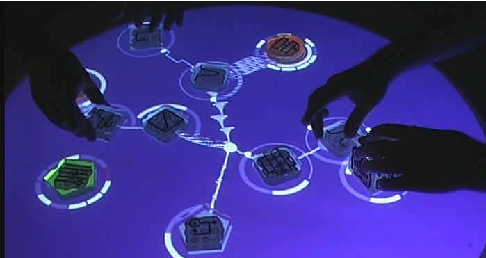
\includegraphics[width=0.47\textwidth]{figures/reactable.pdf}
\caption{The reacTable in action (compare \protect\cite{jorda07})}
\label{fig:reactable}
\end{figure}

Modular synthesis is used for the sound generation process. In reacTable, automatic connections between objects are made depending on the type of objects involved and the proximity between them. By moving objects around and bringing them into relation to each other, performers construct and play instruments at the same time. reacTable is also a collaborative tool for interactive live music. Because of the rather big size of the table-top, multiple artists can use a single reacTable collaboratively. 

Many artists have incorporated reacTable in their performance recently. Because reacTable relies on synthesizers for audio generation, not every musical style can be performed with the TUI. Therefore, reacTable is suited best for electronic styles of music. The interaction techniques seem to be very intuitive and easy to learn, so the system can be used by unexperienced as well as professional users. \cite{jorda07} state that users grasp the basic principle of the reacTable after approximately 5 minutes of unguided interaction. Users with little knowledge of musical theory and synthesis can actually create and perform music with the TUI easily. 

\subsubsection{TARboard}
TARBoard by \cite{lee05} is a tangible augmented reality system designed for table-top game environments. The purpose of TARBoard is is to let users enjoy games in a more interactive and intuitive way and to make games more realistic and immersive.

\begin{figure}
\centering
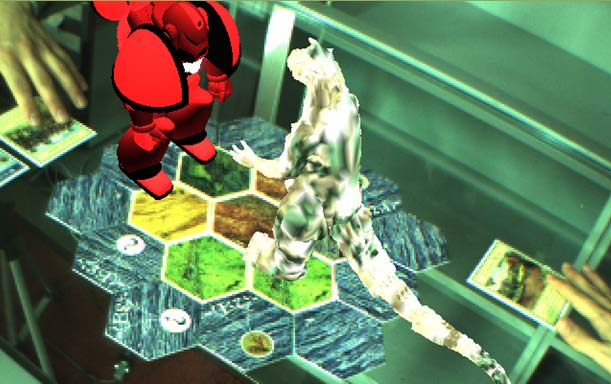
\includegraphics[width=0.47\textwidth]{figures/tarboard.jpg}
\caption{The TARBoard TUI (compare \protect\cite{lee05})}
\label{fig:tarboard}
\end{figure}

Markers are attached to objects or cards used in a game. Similar to reacTable, these markers are tracked on a table-top environment by a camera underneath it. The augmenting camera is placed above the table-top. It provides the video stream for augmenting a game with virtual objects.

\cite{lee05} implemented a card game as a prototype for TARBoard. Each player has cards which represent mystic creatures. The marker on the bottom of each card is tracked by the tracking camera. When the players flip a card and place it near the battle zone, the creatures get augmented on the battle zone and fight against each other. This scenario is shown in figure \ref{fig:tarboard}.

TARBoard seems to be an interesting way of enhancing physical games with virtual features. As a result, physical games could be made more attractive for young people. It would be easy to enhance card games with fiducial markers, but the price of the hardware for tracking and visualizing would remain a problem. 

\subsection{Urban Planning Workbenches}
In urban planning, designers usually employ three forms of representation: Two-dimensional drawings on sheets of papers, three-dimensional physical models and computer models, which can be two and three-dimensional. Each of these representations are created and displayed independently. Urban planning workbenches try to bridge the gap between these forms of representation, by simultaneously layering 2D drawings, 3D physical models, and digital simulations over each other. 
First, the 2D drawings and sketches are laid out on a table. Next, the 3D models are placed on top of the drawings. Finally, video projectors project digital simulations onto the surface. Video cameras capture the activity on the table and adjust the dynamic representation according to the position of the drawings and models with optical tags \cite{ishii02}.

The advantage of urban planning workbenches lies in the combination and fusion of digital and analog content. The dynamic simulation of features like shadows, traffic and wind bring the analog content placed on the workbench to life. Users gain a more thorough understanding of the implications of their designs. Furthermore, the two- and three-dimensional physical representations together with the digital projections add to a more realistic simulation of an urban design space \cite{ishii02}.

\begin{figure}
\centering
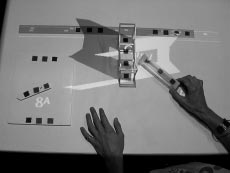
\includegraphics[width=0.47\textwidth]{figures/urp.jpg}
\caption{A building becomes glass in Urp (compare \protect\cite{underkoffler99})}
\label{fig:urp}
\end{figure}

\subsubsection{Urp}
Urp, presented by \cite{underkoffler99} is an implementation of an urban planning workbench. Urp is classified as a luminous-tangible interface. The accurate casting of shadows and reflections of the 3D models is a very important part of the system. The Urp urban planning workbench consists of the following five key functions:
\begin{itemize}
\item Shadows: Urp casts accurate shadows of the 3D models onto the projection table. With a clock object, the user can change the position of the computational sun and see how the shadows of the models change accordingly. 
\item Distance Measurements: With the distance-tool, a line between two buildings can be drawn. The drawn line connects two structures, with the lines length displayed beneath. The number continuously changes as the connected structures are moved. 
\item Reflections: When a user touches any building with a transparent wand, its facades become glassy, so that solar reflections are generated and projected onto the table. Figure \ref{fig:urp} shows this scenario.
\item Wind Effects: Urp is able to project an airflow simulation onto the workbench. The user can choose between eight quantized wind directions. The simulation is displayed as a regular array of white segments, whose direction and length correspond to the instantaneous direction and magnitude of the wind at that position.
\item Site Views: Since the model buildings 3D forms are already resident in the system (because of the shadow generation), they can be rendered in perspective. Placing a camera object in the workspace results in a real-time rendering of the current arrangement of buildings in the site, viewed from the height of a pedestrian and the position and orientation of the camera. 
\end{itemize}
Urp can also simulate traffic on roads, when traffic strips are placed onto the workspace. When two plastic strips cross each other, the simulation creates an intersection with implicit traffic-control signals. Cars come to a halt in one direction, while the traffic in the other direction flows.

\subsubsection{The Luminous Table}
The Luminous Table is based upon the Urp urban planning workbench, but extends its functionality to a more mature form \cite{ishii02}. The Luminous Table software allows more flexibility in the computation of shadows by allowing users to interactively change the latitude (Urp has a fixed latitude) and set the time of the simulation more precisely. The traffic simulation in the Luminous Table is also more advanced compared to Urp. Users can change the road length, road width, traffic density and traffic cycle time of the simulation. Furthermore, the luminous desk supports more geometry formats for models of urban structures and implements the ability to save and restore work. Figure \ref{fig:luminous_table} shows students interacting with the Luminous Table.

\begin{figure}
\centering
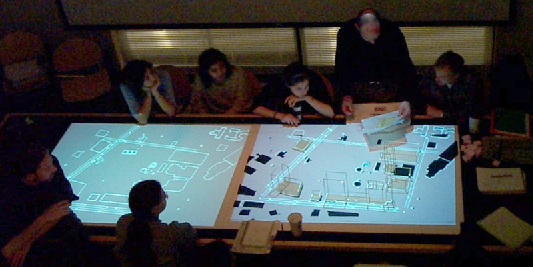
\includegraphics[width=0.47\textwidth]{figures/luminous_table.pdf}
\caption{Students using the Luminous Table (compare \protect\cite{ishii02})}
\label{fig:luminous_table}
\end{figure}

Urban planning workbenches can be very useful tools for architects and urban designers by combining several forms of urban design representations into one simulation. This is not only useful for the urban designers themselves, but also for clients, who can get a clearer understanding of the design prototypes. The visualizations employed in urban workbenches can help solving design implications like shadow casting between different buildings. By taking objects away from the table and putting them onto different places the user can change the planning scene quickly. Different scenes and their simulated implications can be tested fast without using mouse and keyboard interaction.

\subsection {Other forms of Tangible User Interfaces}
There are many other different forms of Tangible User Interfaces for a variety of different devices and application scenarios. We will discuss some of them in the following section. 

\subsubsection{Portico}
Portico is a portable system for enabling tangible interaction on and around tablet computers \cite{avrahami11}. Two cameras mounted on small, foldable arms are positioned above the display to recognize a variety of physical objects. These objects can be placed on the tablet or around it. The cameras have a large field-of-view, so the interaction can be extended beyond the tablet. An illustration of the Portico system can be seen in \ref{fig:portico}. The prototype developed by \cite{avrahami11} uses a 12" inch tablet, but the interaction space is six times the size of the tablet screen. Portico allows tablets to increase both their interaction space and sensing capabilities, without sacrificing portability. Portico can be used for games or educational purposes. Because physical objects are more graspable than touch surfaces, Portico would be suited as a learning device for young children. 

\begin{figure}
\centering
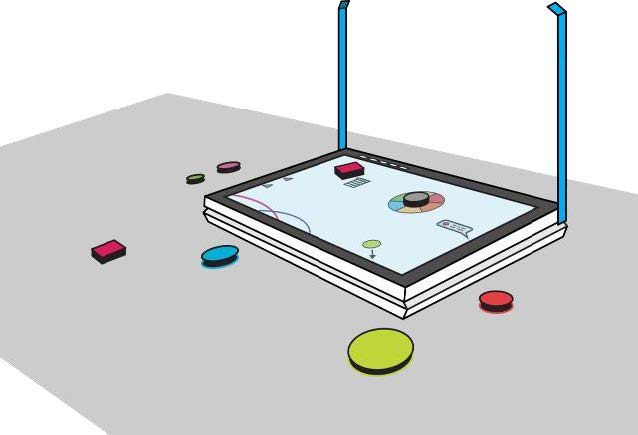
\includegraphics[width=0.47\textwidth]{figures/portico.jpg}
\caption{An illustration of the Portico system (compare \protect\cite{avrahami11})}
\label{fig:portico}
\end{figure}

\subsubsection{Paper Windows}
Paper Windows, a TUI introduced by \cite{holman05}, simulate the use of digital paper displays by projecting digital content onto physical paper. IR cameras track the motion and the shape of the paper for an accurate projection. Pens, fingers, hands and other objects are also tracked by the computer vision system to allow enhanced interaction with the paper documents. \cite{holman05} introduce a set of new interaction techniques to allow interactions between different paper documents. The rubbing technique for example allows users to transfer contents between paper documents. The flipping interaction allows users to navigate through the document by flipping the paper in their hands. Paper can also be stacked to organize them in piles on a desk. On the paper document itself, items can be selected through a one handed pointing gesture. Interactions like Copy \& Paste, Scrolling, Browsing and Sharing are also possible.

The strength of Paper Windows lies in the presence of multiple displays for parallel activities. Therefore, several tasks can be done simultaneously. This is shown in figure \ref{fig:paperwindows}, where several Paper Windows are laid out. By using the provided gestures, users can exchange information between Paper Windows. A possible scenario for Paper Windows shown by \cite{holman05} is the composition of a photo collage. The user can search through photo thumbnails provided by one Paper Window. He can put together a collection of photos by simply swiping interesting photos onto another Paper Window with his finger.

\begin{figure}
\centering
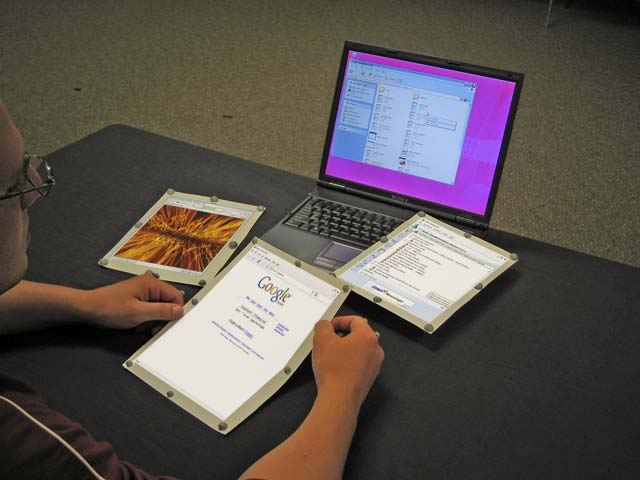
\includegraphics[width=0.47\textwidth]{figures/paperwindows.jpg}
\caption{Paper Windows in a possible usage scenario (compare \protect\cite{holman05})}
\label{fig:paperwindows}
\end{figure}

\subsubsection{3D Tractus}
\cite{lapides00} present a three-dimensional user interface to monitor and control a team of independent robots in a spatial tasks. The 3D Tractus is a tangible user interface, which allows to change the height in a three-dimensional environment. It is a mechanical device consisting of a table surface that slides up and down on four vertical tracks. A tablet is placed on top of the table surface to control a 2D map. The user can move the table surface up and down to change the height in the environment. The purpose of the system is to control a robotic team inside a three-dimensional building, where a bomb has to be defused. A single human operator controls multiple robots by giving them instructions on the tablet PC. The tablet provides a topdown view of the building.